\section{Empirical Evaluation Protocol}

This thesis is based on the empirical analyses to measure the energy consumption. As we mentioned earlier, we have chosen the \emph{agile} methode. so basically we will reduce the energy consumption with trial and error. 


%%%%%%%%% preliminary taughts and section structure 
% The need of reproducibility in our field - software optimization based on empirical studies -

% The importance of Virtualisation for reproducibility \cite{howe_virtual_2012}
% some of the most important parts are
% - fewer constraints on research methods
% - on-demand backups
% - virtual Machines as Publications
% - more Variables captured
\subsection{Threats and Challenges}


One of the most challenges which face the reaserchers is the reproducibility of their tests.Actually many results are not reproducible \footnote{Trouble at the lab, The Economist, 19 October 2013;  www.economist.com/news/briefing/ 21588057-scientists-think-science-self-correcting- alarming-degree-it-not-trouble.}, which let to a \emph{replication crisis}.When this crisis hit most of the empirical studies,most of the reviews now includes reproducibility as one of the minimal standard for judging scientific \cite{peng2011reproducible}. one of the creterions for a reproducidibility is the publication of the dataset and the algorithm run on the raw data to condlude the results. There is even some disagreement about what the terms "reproducibility" or "replicability" by themselves mean \cite{goodman2016does} .According to \cite{echtler2018open} \emph{replicability} extends \emph{reproducibility} to the ability to collect a new raw dataset comparable to the original one by reexecuting the experiment under similar condition, Instead of just the ability to get the same results by ruruning the statistical analyses on the orginal data set.

One major problem that hinders the reproducibility of the empirical tests is the interaction with the external environment, either as concurency or dependencies. Therefore testers won't have the same results unless they duplicate the same environment.
% introduction of vms 
\subsection{Virtualisation}
To resolve this problem, practitioners tend to use Virtualisation. Using virtual machines aka VM gives reaserchers the freedom to choose their own tools, software and operating system that they are the most confortable with without paying the price to change the actual working environment, which will give them eventually more controle over the dependencies and the execution environement. Moreover, using a vm will solve the \emph{replication crisis} thanks to the virtual images, even the most complex architecture can be reproduced easily by just instantiating a copy of the image. Since the virtual machines are agnostic to the host architecture, reaserchers won't have to worry about where and how their experiments are replicated because they have already setup the execution environement. Another advantage to the virtual machines is the snapshot mechanism, it allows reaserchers to create backups and revert some changes with simple clicks. Last but not least,thanks to the isolation, virtual machines push the reproducibility further by allowing the future usages to see all the variables -controled and uncontroled-  and do other analysis without dealing with any dependencies. In his paper \cite{howe_virtual_2012} bill howe lists the advantages of using virtual machines in reaserchers experements including the economical impact and cultural limitation to a such approach.

which allow them to have control over the ressouces, the dependencies and the execution environment. Moreover, thanks to the snapshots, deploying a software is easily done by instantiating a copy of that image.
However, this choice comes with a certain cost. Because the intervention of the hypervisor,the software will use two kernels , the virtual machine one and the host machine one, which will provide a noticiable overhead, and will impact the performances of the tests.Therefore, we can't use virtual machines for exepements that are related to performance. Another limiation with the virtual machine is the the isolation. It is true that this feature will prevent the experience environement with any undesirable interference from the outside world. but sometimes this contact is needed, especially when the experiment is dependent to an external part, such as sensors. In energicial tests we tend to use hardware powermeters which will make it difficult to use the virtual machines in this case .

% introduction of docker 

\begin{figure}
    \center{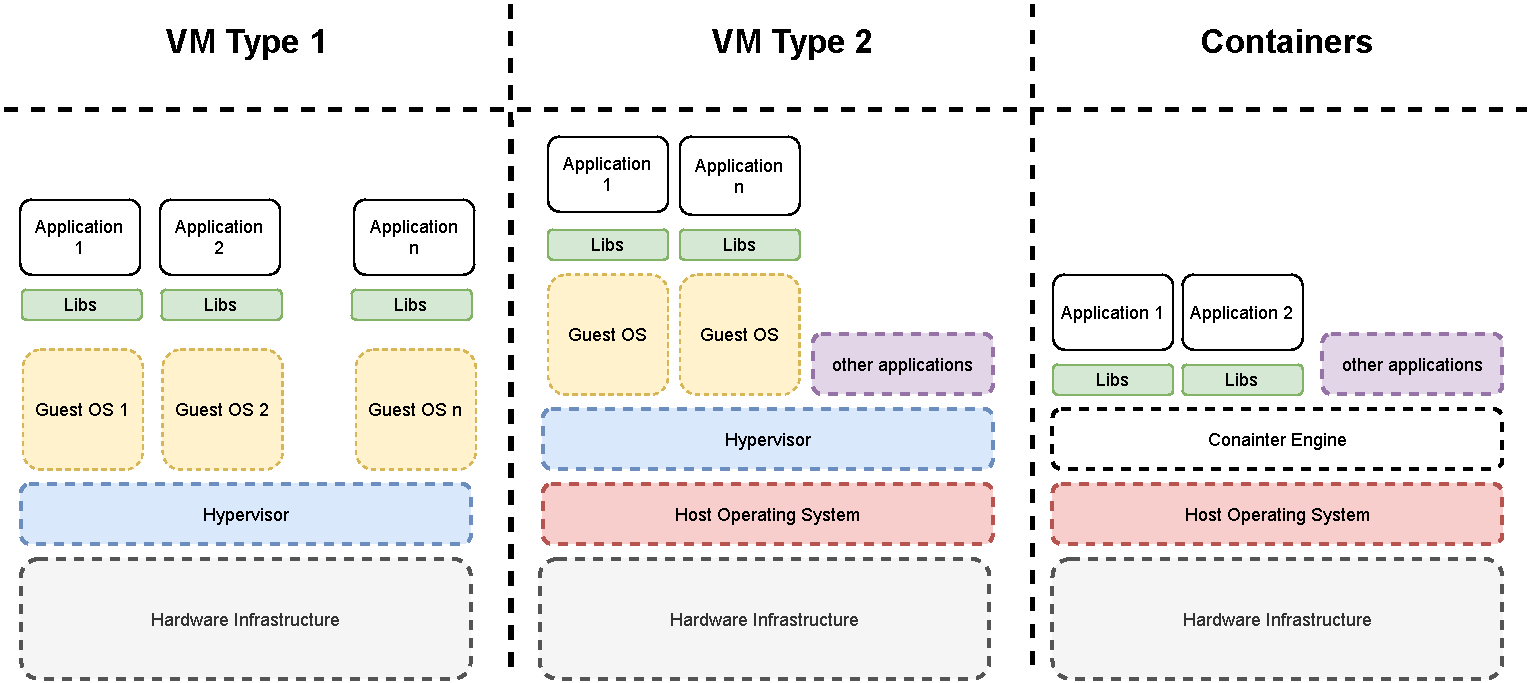
\includegraphics[width=1\linewidth]{imgs/virtualization_techniques}}
    \caption{Different Methods of Virtualzation}\label{reproducibility:virtualization_technique}
\end{figure}

\subsection{Containers}

another solution would be using something that allows us to have the isolation from the host os and the ease of replication that virtual machines offer, and the direct interaction with the hardware that the classical method give.
contarization offers a such advantages while keeping the isolation and the ease of replication for application.

Figure \ref{reproducibility:virtualization_technique} explains the differents in architecture between the clasic types2 of Virtualisation and Containers.
\begin{itemize}
    \item Type 1: runs directly on the hardware, it is mainly used by the cloud providers where there is no main OS, but just virtaul machines, we can site for this the open-srouce XEN and VMware ESX
    \item Type 2: runs over the hostmachine Operating System, mostly used for personal comptuers, VMware server and virtualBox are famous examples of this type, most of the reaserchers expermentation are run witht this type, howerver due to the 2 Operatings syestms the applications tend to be more slower
    \item containers : Instead of its own kernel, containers used the hots kernel to run their Os, which makes them ligher, quickers and use the full pontial use of the hardware. For this we can cite \emph{Docker}, \emph{Linux LXC}\emph{LXD} \cite{abuabdo_virtualization_2019}
\end{itemize}
\note{Rephrase so i include it before VMs+ add links to the technologies }


\subsection{Docker vs Virtual Machine}
Depsite that Type 1 is more performant than type 2, the second one is the most used in reaserch, since most researchers conducts their experements in their own machine. In the other hand, docker is the most famous thechonology for for containers,

%%%%% THINGS TO ADD : 
% the impact of docker on the reprodudicibility 
% Limits of docker 
% The docker files and the clarification of the methodology 

\subsection{Docker and energy}
%  basically just rephrase the paper 


\subsection{docker and accuracy}





\subsection{Testing Protocol}
the results of this protocil can be found in the project of the continious integrtation that was made by the intern Mamadou to give a feedback about the evolution of the energyconsumption within time


